% *********************************************************************
% © 2021-2023 Jeremy Sylvestre
%
% Permission is granted to copy, distribute and/or modify this document
% under the terms of the GNU Free Documentation License, Version 1.3 or
% any later version published by the Free Software Foundation; with no
% Invariant Sections, no Front-Cover Texts, and no Back-Cover Texts. A
% copy of the license is included in the appendix entitled “GNU Free
% Documentation License” that appears in the output document of this
% PreTeXt source code. All trademarks™ are the registered® marks of
% their respective owners.
%
% *********************************************************************

\newcommand*{\xmin}{-0.5}
\newcommand*{\xmax}{6.5}
\newcommand*{\ymin}{-6.5}
\newcommand*{\ymax}{10}

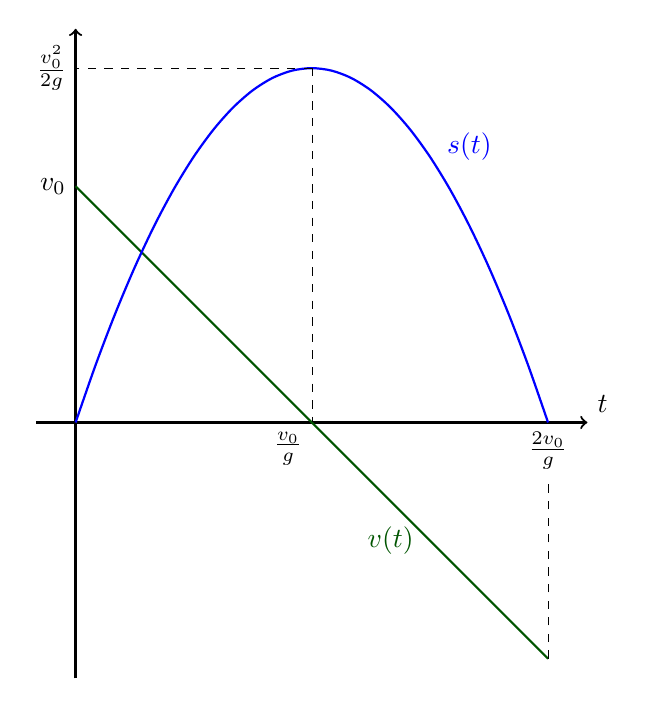
\begin{tikzpicture}
[
	closedpt/.style={circle,draw,fill,inner sep=0pt,minimum size=4pt},
	openpt/.style={circle,draw,inner sep=0pt,minimum size=4pt},
	yscale=0.5
]

	% v0 = 6, g = 2

	% axes
	\draw[->,thick] (\xmin,0) -- (\xmax,0) node[above right] {$t$};
	\draw[->,thick] (0,\ymin) -- (0,\ymax);

	% velocity
	\draw[green!33!black,thick] (0,6) -- (6,-6);
	\node[green!33!black] at (4,-3) {$v(t)$};

	% position
	\draw[blue,thick,domain=0:6,smooth] plot (\x,{- \x * \x + 6 * \x});
	\node[blue] at (5,7) {$s(t)$};

	\node[below] at (6,0) {$\frac{2 v_0}{g}$};
	\draw[dashed, very thin] (3,9) -- (3,0) node[below left] {$\frac{v_0}{g}$};
	\draw[dashed, very thin] (6,-6) -- (6,-1.5);

	\node[left] at (0,6) {$v_0$};
	\draw[dashed, very thin] (3,9) -- (0,9) node[left] {$\frac{v_0^2}{2 g}$};


\end{tikzpicture}
